\documentclass[11pt,a4paper]{article}

%% -------------------------------
%% NCI MSc Research Project Template      
%% -------------------------------


% ----------------------------------------------------------------
% Report - Main document
% ----------------------------------------------------------------

%Project Type Switch -- change this if and only if you are doing an industry Internship
\newif\ifindustry

\industryfalse
% \industrytrue

%% ---------------------------------
%% |      Additional packages      |
%% ---------------------------------

\usepackage[british,UKenglish]{babel}  %% Language
\usepackage[a4paper, margin=1in]{geometry} %% margins
%% \usepackage{cite} must not be loaded alongside natbib - natbib warns about it
%% and the two redefine \cite against each other. natbib's `sort' option does
%% the job cite was providing.
\usepackage[sort]{natbib} %% References -- Harvard referencing style
\usepackage{graphicx} %http://en.wikibooks.org/wiki/LaTeX/Importing_Graphics#Graphics_storage
\usepackage[export]{adjustbox}
\usepackage[absolute,overlay]{textpos}
\usepackage{tikz}
\usepackage{algorithm} % Code-Listings
\usepackage{algorithmic} % Code-Listings
% see http://www.ctan.org/tex-archive/macros/latex/contrib/algorithm2e/algorithm2e.pdf
% for more sophisticated algorithm listings
\usepackage{amsmath,amsfonts,amssymb}	% AMS mathematical facilities, fonts and symbols
\usepackage{lastpage}
\usepackage{datetime}
%% Harvard citation punctuation. natbib driving dcu.bst otherwise separates the
%% author from the year with a semicolon - '(Lewis et al.; 2020)' - which is not
%% Harvard. This restores '(Lewis et al., 2020; Shuster et al., 2021)'.
\bibpunct{(}{)}{;}{a}{,}{,}

%% --- added for this report: booktabs rules, p-column modifiers, caption styling
\usepackage{booktabs}
\usepackage{array}
\usepackage{caption}
\usepackage{microtype}
\captionsetup{font=small,labelfont=bf,skip=5pt,belowskip=3pt}
\renewcommand{\arraystretch}{1.12}
%% Let floats fill more of a page before LaTeX defers them, so a table near a page
%% break does not push over and leave a band of white space behind it.
\renewcommand{\topfraction}{0.92}
\renewcommand{\bottomfraction}{0.80}
\renewcommand{\textfraction}{0.06}
\renewcommand{\floatpagefraction}{0.80}
\setcounter{topnumber}{3}
\setcounter{totalnumber}{5}
\setlength{\textfloatsep}{10pt plus 2pt minus 2pt}
\setlength{\intextsep}{10pt plus 2pt minus 2pt}
%% 31 Harvard entries at full size and full leading run to three pages alone. The
%% reference list is scanned rather than read, so it carries the compression.
\setlength{\bibsep}{1pt plus 0.2ex}
\renewcommand{\bibfont}{\footnotesize}
\usepackage[bookmarks=true, colorlinks=false]{hyperref} % Links - must be last package

\DeclareGraphicsExtensions{.pdf,.png,.jpg}
\graphicspath{{./figures/}} %Use curly braces for each path to add 

%% ---------------------------------
%% | Information about the report  |
%% ---------------------------------

% Uncomment one of the following, according to your module name
\newcommand{\mytype}{MSc Research Project}
%\newcommand{\mytype}{MSc Research Project}
%\newcommand{\mytype}{MSc (Research) Practicum}
%\newcommand{\mytype}{MSc Internship}

% Uncomment one of the following, according to your programme
\newcommand{\mystream}{Artificial Intelligence}
%\newcommand{\mystream}{Cloud Computing}
%\newcommand{\mystream}{Data Analytics}
%\newcommand{\mystream}{Cybersecurity}
%\newcommand{\mystream}{Artificial Intelligence}
%\newcommand{\mystream}{Artificial Intelligence for Business}
%\newcommand{\mystream}{FinTech}
%\newcommand{\mystream}{Open Data Practice}


\newcommand{\myname}{Mastan Vali Shaik}
\newcommand{\studentID}{24226807}
\newcommand{\mytitle}{Personalised Medical Question Answering: A Matched-Prompt Comparison of Neural Retrieval, a Large Language Model, and a Retrieval-Augmented Hybrid}

\newcommand{\supervisor}{Devanshu Anand}
\newcommand{\supervisortwo}{} % for Internship with a clear supervisor only!


%% -------------------------------
%% |  Information for PDF file   |
%% -------------------------------
%% Auto-Fill this information
\hypersetup{
 pdfauthor={\myname},
 pdftitle={\mytitle},
 pdfsubject={\mytype},
 pdfkeywords={\mystream}
}

%% ---------------------------------
%% | ToDo Marker - only for draft! |
%% ---------------------------------
% Remove all \todo instances for the final version!
\setlength{\marginparwidth}{20mm}

\newcommand{\margtodo}
{\marginpar{\textbf{\textcolor{red}{ToDo}}}{}}

\newcommand{\todo}[1]
{{\textbf{\textcolor{red}{(\margtodo{}#1)}}}{}}


% Describe separation hints here:
\hyphenation{
per-son-al-i-sa-tion
hal-lu-ci-na-tion
re-triev-al
aug-men-ta-tion
bi-di-rec-tion-al
di-men-sion-al
re-pro-duc-i-ble
}

%% TeX will not hyphenate the parts of an already-hyphenated compound, and this
%% report is full of them ("128-dimensional", "retrieval-augmented"), which
%% leaves the occasional line marginally overfull. \emergencystretch is only
%% consulted for paragraphs TeX cannot otherwise set, so it costs nothing
%% elsewhere.
\emergencystretch=1em


%% ------------------------
%% |    Including files   |
%% ------------------------
% Every section is pulled in with \input below, so no \includeonly filter is
% needed. Leaving one in place risks silently dropping a section if the list
% and the \input calls ever drift apart.

%%%%%%%%%%%%%%%%%%%%%%%%%%%%%%%%%
%% Here, main documents begins %%
%%%%%%%%%%%%%%%%%%%%%%%%%%%%%%%%%
\begin{document}

\include{titlepage}

%% -----------------
%% |   Main part   |
%% -----------------

\title{\mytitle}%
%\author{\myname \\ \studentID \\ \mytype\ in \mystream}%
\author{\myname \\ \studentID}%
\date{}
\maketitle

\pagestyle{plain}
\pagenumbering{arabic}

\begin{abstract}

Background: Patients with long-term health conditions often receive detailed advice during medical consultations but have limited support once they return home. Medical question answering systems can help bridge this gap. Retrieval-based systems usually provide reliable information from trusted sources, but the responses are often generic and do not consider the patient's individual circumstances. Large language models can generate personalised answers, although they may sometimes produce information that is not supported by reliable medical evidence.

Objectives: This study truly investigates whether combining a neural retrieval model with a large language model improves the quality of personalised medical question answering compared with using either approach independently. It also examines the conditions under which retrieval augmentation is most effective.

Methods: Three medical question answering systems that were developed using 3,000 question--answer pairs from the MedQuAD dataset. The first system combined a Siamese BiLSTM retriever with a rule-based response module. The second used Gemini 3.5 Flash Lite to generate responses directly from the user's question. The third was a hybrid Retrieval-Augmented Generation (RAG) system that combined retrieval with the language model. Both language-model systems used the same base prompt so that retrieval was the only experimental difference. Responses were evaluated by an independent model (Gemini 3.1 Flash Lite) using a four-axis clinical rubric. The generated answers were also reviewed through claim-level verification, and pairwise statistical comparisons were performed using Holm correction.

Results: After correcting the five implementation issues in the retriever, Recall@1 improved from 0.010 to 0.513. An ablation experiment showed that a worked example included in the original evaluation rubric unintentionally limited scores to a maximum of 78, making the earlier finding unreliable (p = 0.766). When relevant information was available in the knowledge base, the hybrid system achieved the highest overall score (79.3), followed by the standalone language model (78.2) and the retrieval-only system (49.0). The hybrid approach also reduced hallucinated medical statements by 16\%, although this difference was not statistically significant. When the supporting document was removed from the knowledge base, the advantage of retrieval augmentation disappeared.

Conclusions: The results indicate that retrieval augmentation improves the factual reliability of medical question answering when relevant information is available in the knowledge base. Its main benefit is improving faithfulness rather than producing more fluent responses. The study also highlights the importance of carefully designing evaluation prompts, as even a single example included in the judging rubric can influence the final evaluation.

Keywords: medical question answering; retrieval-augmented generation; BiLSTM; personalisation; hallucination; LLM-as-a-Judge; MedQuAD.

\end{abstract}

\section{Introduction}
\label{sec:Introduction}

\subsection{Background and Motivation}

Long-term health conditions account for a large proportion of healthcare services in developed countries. Patients with conditions such as type 2 diabetes and hypertension manage their health every day by monitoring symptoms, taking medication, and deciding when medical attention is needed. Since medical consultations are usually short and infrequent, many of these decisions are made without immediate professional support.

Large language models (LLMs) have created new opportunities for conversational medical assistants. They can generate fluent and natural responses, making them suitable for medical question answering. However, in healthcare, fluency alone is not enough. Responses must also be accurate, relevant to the patient, and safe when the model is uncertain. Incorrect medical information may have serious consequences.

\citet{ji2023} showed that LLMs can generate convincing but incorrect information, while \citet{thirunavukarasu2023} argued that the main challenge in clinical deployment is verifying the reliability of generated responses. These limitations highlight the need for approaches that improve factual accuracy without losing the benefits of natural language interaction.

\subsection{Problem Statement}

Medical question answering systems generally follow one of two approaches. Retrieval-based systems return information from trusted medical documents, making them reliable but often unable to personalise responses. In contrast, large language models generate personalised answers but may produce unsupported or incorrect medical information.

Retrieval-Augmented Generation (RAG) combines these approaches by providing the language model with relevant documents before generating a response \citep{lewis2020}. Although RAG has shown promising results, its effectiveness in medical question answering is still uncertain.

\citet{xiong2024} found that retrieval improves responses only when relevant information is available, while \citet{gao2024} observed that many studies focus mainly on successful retrieval cases and rarely evaluate situations where retrieval fails.

Evaluating medical question answering systems is another challenge. Traditional text-overlap metrics do not measure clinical usefulness or personalisation, while LLM-based evaluation introduces its own biases. Therefore, both the systems and their evaluation methods require careful assessment.

\subsection{Research Question and Objectives}

This study investigates the following research question:

\textbf{Does a hybrid medical question answering system that combines a BiLSTM retriever with a large language model produce better patient-focused responses than retrieval or generation alone, and does its performance depend on knowledge-base coverage?}

The objectives of this study are to:

\begin{enumerate}

\item Train a Siamese BiLSTM retriever using the MedQuAD dataset and evaluate it with standard retrieval metrics.

\item Develop three comparable medical question answering systems using the same base prompt so that retrieval is the only experimental difference.

\item Evaluate response quality using an independent language model and a structured clinical rubric.

\item Perform claim-level verification to identify hallucinated information, including incorrect numerical values.

\item Compare the systems using statistical significance testing with multiple-comparison correction.

\item Investigate how knowledge-base coverage influences the performance of Retrieval-Augmented Generation.

\end{enumerate}

Performance is evaluated using Recall@1 for retrieval, rubric scores with bootstrap confidence intervals for response quality, claim-level hallucination rates for factual accuracy, and Holm-corrected paired statistical tests for system comparisons.

\subsection{Contribution}

This study makes three main contributions.

First, it demonstrates that including a worked example in an LLM-as-a-Judge prompt can unintentionally bias evaluation scores. This explains why an earlier version of the project reported a positive finding that disappeared after the evaluation procedure was corrected.

Second, it presents a corrected and properly evaluated neural retriever. Fixing five implementation issues improved Recall@1 from 0.010 to a level that outperformed the TF-IDF baseline.

Third, it provides a controlled comparison of retrieval-only, language-model-only, and Retrieval-Augmented Generation systems under different knowledge-base coverage conditions. The results show that retrieval augmentation improves factual reliability when relevant documents are available but provides limited benefit when they are not.

\subsection{Structure of the Report}

This report is organised into eight sections.

Section 2 reviews the literature and identifies the research gap. Section 3 describes the research methodology. Section 4 presents the system design, and Section 5 explains the implementation. Section 6 summarises the project outputs. Section 7 presents the experimental results and critical analysis. Finally, Section 8 concludes the study and discusses future work.

\section{Literature Survey}
\label{sec:Relatedwork}

\subsection{Sequence Encoders and Dense Retrieval}

Long Short-Term Memory (LSTM) networks solved the vanishing gradient problem, allowing recurrent models to learn long-range dependencies \citep{hochreiter1997}. Bidirectional LSTMs further improved sentence representation by processing text in both directions, while the Gated Recurrent Unit (GRU) provided a simpler alternative with fewer parameters \citep{cho2014}. The introduction of the Transformer architecture \citep{vaswani2017} shifted natural language processing away from recurrent networks through self-attention, and BERT \citep{devlin2019} established contextual language modelling as the standard approach. BioBERT later adapted this framework for biomedical applications \citep{lee2020}.

Dense retrieval represents both queries and documents as vector embeddings instead of relying on keyword matching. \citet{reimers2019} demonstrated that Siamese sentence encoders can generate effective semantic embeddings, while \citet{karpukhin2020} showed that Dense Passage Retrieval outperformed the traditional BM25 ranking method \citep{robertson2009} on open-domain question answering.

Several implementation details have a significant impact on retrieval performance. Pooling operations should exclude padding tokens, negative sampling should encourage meaningful discrimination between documents, and contrastive objectives such as InfoNCE improve embedding quality by treating other batch samples as negatives \citep{oord2018}. Vocabulary handling is also important because mapping unknown medical terms to the padding index can remove critical clinical information. Although these issues appear minor individually, they can substantially reduce retrieval performance, as demonstrated later in Section 7.2.

\subsection{Retrieval-Augmented Generation and Medical Question Answering}

Retrieval-Augmented Generation (RAG) combines document retrieval with language generation by supplying external evidence during response generation \citep{lewis2020}. In healthcare, this approach is particularly valuable because medical advice requires reliable and traceable sources. \citet{zakka2024} applied this principle in Almanac by grounding responses in clinical guidelines, while \citet{li2023} proposed ChatDoctor through model fine-tuning without external retrieval. \citet{singhal2023} further demonstrated that large language models can encode substantial medical knowledge through Med-PaLM.

The effectiveness of RAG depends on the availability of relevant documents. \citet{xiong2024} reported that retrieval improves answer quality only when the knowledge base contains suitable information, whereas irrelevant documents may reduce performance. \citet{gao2024} reached a similar conclusion, noting that knowledge-base coverage is rarely evaluated explicitly. \citet{shuster2021} showed that retrieval can reduce hallucinations in dialogue systems, while \citet{guu2020} proposed REALM, which jointly learns retrieval and generation but reduces the flexibility of updating external knowledge.

Personalisation remains less explored than factual correctness. Most personalised healthcare systems rely on structured patient profiles, whereas existing medical question answering benchmarks evaluate generic responses rather than patient-specific advice. As a result, current benchmarks rarely assess whether answers consider a patient's medical history, existing conditions, or medications. This limitation motivates the personalised evaluation adopted in this study.

\subsection{Evaluating Generated Clinical Text}

Traditional evaluation metrics such as ROUGE \citep{lin2004} and BLEU \citep{papineni2002} measure similarity between generated and reference text. However, these metrics are less suitable for personalised medical question answering because responses that correctly include patient-specific information may differ substantially from generic reference answers.

To address this limitation, \citet{zheng2023} introduced LLM-as-a-Judge, demonstrating that language models can evaluate generated responses with reasonable agreement to human judgement while also highlighting known sources of bias. Similarly, \citet{es2024} proposed RAGAS, which evaluates retrieval-augmented systems using measures such as faithfulness and relevance.

This study combines both approaches while reducing their limitations. Response quality is evaluated using an independent language model together with claim-level verification, ensuring that important conclusions are supported by both automated evaluation and direct evidence. The study also identifies an additional source of evaluation bias, showing that including a numerical example in the judging rubric can unintentionally influence the scores assigned by the evaluation model.

\subsection{Comparison of Related Systems and the Research Gap}

Table 1 compares this study with six representative works. It examines whether previous studies evaluate patient-specific profiles, perform claim-level grounding audits, and consider knowledge-base coverage as an experimental factor.

\refstepcounter{table}
\label{tab:1}
\begin{center}
\scriptsize
\setlength{\tabcolsep}{3pt}
\begin{tabular}{>{\raggedright\arraybackslash}p{0.145\textwidth}>{\raggedright\arraybackslash}p{0.211\textwidth}>{\raggedright\arraybackslash}p{0.094\textwidth}>{\raggedright\arraybackslash}p{0.085\textwidth}>{\raggedright\arraybackslash}p{0.106\textwidth}>{\raggedright\arraybackslash}p{0.234\textwidth}}
\toprule
\textbf{Study} & \textbf{Evaluation} & \textbf{Profile} & \textbf{Claims} & \textbf{Coverage} & \textbf{Limitation addressed here} \\
\midrule
Lewis et al. (2020) & EM / F1 & No & No & No & Introduced RAG but evaluates factoid accuracy only. \\
Karpukhin et al. (2020) & Recall@k & No & No & No & Retrieval quality only; no generation or safety analysis. \\
Li et al. (2023) & BLEU / human & No & No & No & Fine-tuning, not retrieval; no per-claim grounding audit. \\
Singhal et al. (2023) & Accuracy / panel & No & Partial & No & Clinician panel, but exam questions and no patient profile. \\
Zakka et al. (2024) & Clinician rating & No & Yes & No & Closest work; grounds in guidelines but does not personalise. \\
Zheng et al. (2023) & Pairwise preference & No & No & No & Establishes judge methodology; documents position/self bias. \\
This work (2026) & Blind 4-axis rubric, claim-level audit, IR metrics & Yes & Yes & Yes & - \\
\bottomrule
\end{tabular}
\end{center}

Table 1 shows three important research gaps. First, most medical question answering studies evaluate answers to questions rather than answers tailored to individual patients. As a result, responses that ignore a patient's medical history or medications are often scored the same as personalised responses. Second, faithfulness is commonly measured using text-overlap metrics or overall human judgement instead of verifying individual claims against supporting evidence. Third, knowledge-base coverage is usually assumed rather than evaluated, even though \citet{xiong2024} showed that retrieval performance depends heavily on whether relevant information is available.

This study addresses these limitations by introducing patient-specific evaluation, claim-level verification, and knowledge-base coverage as an experimental variable. It also ensures a fair comparison by using the same base prompt for both language-model systems so that retrieval is the only difference between them.

\subsection{Synthesis: The Gap and How This Study Fills It}

The reviewed literature shows that retrieval augmentation can improve factual accuracy \citep{lewis2020,shuster2021}, that large language models already contain considerable clinical knowledge \citep{singhal2023}, and that grounding responses in trusted medical guidelines is feasible \citep{zakka2024}. However, previous studies do not clearly demonstrate how retrieval affects personalised medical question answering when prompt wording is controlled or when the knowledge base does not contain the required information.

Table 2 summarises the main limitations identified in the literature, how this study addresses each limitation, and where the supporting experimental evidence is presented.

\refstepcounter{table}
\label{tab:2}
\begin{center}
\scriptsize
\setlength{\tabcolsep}{4pt}
\begin{tabular}{>{\raggedright\arraybackslash}p{0.368\textwidth}>{\raggedright\arraybackslash}p{0.389\textwidth}>{\raggedright\arraybackslash}p{0.159\textwidth}}
\toprule
\textbf{Gap identified in the literature} & \textbf{How this study addresses it} & \textbf{Evidence} \\
\midrule
G1. Answers are evaluated against questions, not against patients, so ignoring a patient's comorbidities carries no penalty. & A dedicated personalisation axis (0-25) with per-band descriptors, scored blind against a fixed structured profile. & Section 7.3, Table 6 \\
G2. Faithfulness is judged holistically or by n-gram overlap, neither of which localises an unsupported statement. & Every response decomposed into claims and each checked against the evidence pool, with an exact check on doses and other numbers. & Section 7.3, Table 6 \\
G3. Knowledge-base coverage is assumed rather than manipulated, so published gains may hold only on retrieval-friendly questions. & Coverage run as an experimental factor: the same questions answered with and without the answering document in the index. & Section 7.4, Table 7 \\
G4. Retrieval and prompt wording are confounded, because the augmented system and its baseline rarely share a prompt. & One base prompt shared verbatim by both language-model systems; the hybrid adds only the clause governing use of evidence. & Section 3.2, Section 7.3 \\
G5. Neural retrievers are frequently reported through downstream text-overlap scores that cannot separate relevance from fluency. & Retriever measured directly with Recall@k and MRR against a TF-IDF baseline before it is allowed into the pipeline. & Section 7.2, Table 5 \\
G6. LLM-as-judge results are seldom corroborated, despite documented judge biases. & Judge drawn from a different model version than the generator, its rubric ablated for anchoring, and every claim audited by a non-LLM instrument. & Section 7.1, Table 4 \\
\bottomrule
\end{tabular}
\end{center}

Among these limitations, two are particularly important. The first is the use of a shared prompt for both language-model systems, ensuring that retrieval is the only experimental difference. The second is the knowledge-base coverage experiment, which evaluates system performance both with and without the relevant supporting document. These design choices allow the contribution of retrieval augmentation to be measured more reliably.

Overall, this study addresses a methodological gap by providing a controlled comparison of retrieval-only, language-model-only, and hybrid Retrieval-Augmented Generation systems using patient-specific evaluation, claim-level verification, and controlled knowledge-base coverage.

\section{Research Methodology}
\label{sec:Methodology}

This study follows the CRISP-DM framework \citep{wirth2000}, adapted for a comparative evaluation. Business understanding and data understanding are covered in Sections 1 and 3.1, data preparation and modelling in Sections 3.2--4, and evaluation in Section 7. A within-subjects design is used, where every system answers the same questions for the same simulated patient. This allows paired statistical comparisons while reducing variation caused by different test cases.

\subsection{Dataset and Preparation}

The MedQuAD dataset \citep{abacha2019} contains medical question-answer pairs collected from trusted National Institutes of Health sources. Answers shorter than 60 characters were removed, and 3,000 pairs were randomly selected using a fixed seed. The dataset was divided into training (70\%), validation (10\%), and testing (20\%) sets.

For retrieval, all text was converted to lowercase and punctuation was removed. Original formatting was preserved for responses presented to users and the evaluation model.

A single simulated patient profile was used throughout the study: a 45-year-old patient with diabetes and hypertension taking metformin and lisinopril. Keeping the profile constant ensured that differences in performance resulted from the systems rather than changes in patient information.

\subsection{Systems Compared}

Three systems were evaluated.

\textbf{System 1 (ML Only)} used a BiLSTM retriever followed by an extractive rule-based response generator. The retriever selected the most relevant passage, while the rule-based component extracted important sentences and added safety advice when required.

\textbf{System 2 (Gemini Only)} generated responses using Gemini 3.5 Flash Lite based only on the user question and patient profile.

\textbf{System 3 (Hybrid)} combined retrieval with language generation. Up to three relevant passages were retrieved, summarised, and supplied to Gemini together with the patient profile before generating the final response.

Systems 2 and 3 shared the same base prompt. The only difference was the inclusion of retrieved evidence in the hybrid system. The generation temperature was fixed at zero to ensure reproducible outputs.

\subsection{Knowledge-Base Coverage Conditions}

Two experimental conditions were evaluated.

In the \textbf{full-coverage} condition, the complete knowledge base was available during retrieval, representing a realistic deployment scenario.

In the \textbf{leave-one-out} condition, the source document corresponding to each question was removed before retrieval. This ensured that no direct answer was available and allowed the effect of limited knowledge-base coverage to be evaluated.

\subsection{Evaluation Metrics}

Retrieval performance was evaluated using Recall@1, Recall@5, Recall@10, and Mean Reciprocal Rank (MRR), treating the original source document as the relevant result.

Response quality was evaluated by Gemini 3.1 Flash Lite using four criteria: grounding (30), personalisation (25), helpfulness (25), and safety (20). The evaluator was unaware of which system generated each response.

Faithfulness was measured independently through claim-level verification. Each response was divided into individual claims and compared with the supporting evidence. Numerical values such as medication doses and frequencies were checked for exact agreement.

\subsection{Statistical Analysis}

System comparisons were performed using paired t-tests together with Wilcoxon signed-rank tests. Holm correction \citep{holm1979} was applied to control the family-wise error rate across multiple comparisons. Cohen's d \citep{cohen1988} was used to measure effect size, while bias-corrected bootstrap confidence intervals with 5,000 resamples were calculated for all mean scores \citep{efron1993}. Reporting both statistical significance and effect size provides a more reliable interpretation of system performance.

\subsection{Ethical Considerations and Threats to Validity}

This research did not involve human participants or real patient data. The patient profile was synthetic, and the MedQuAD dataset is publicly available. The developed system is intended solely as a research prototype and is not suitable for clinical use.

Several limitations should be considered. Although a different Gemini model was used for evaluation, LLM-based judges may still introduce bias \citep{zheng2023}. Prompt settings were tuned using an initial subset of the data before evaluation on a separate held-out set. In addition, using a single simulated patient profile limits the generalisability of the personalisation results. Finally, the relatively small dataset means that knowledge-base coverage varies across questions, which is why coverage is treated as an experimental factor in this study.

\section{Design Specification}
\label{sec:Design}

\subsection{Architectural Overview}

The proposed system follows an eight-stage pipeline. MedQuAD question-answer pairs are first cleaned and prepared to create the working corpus. Vocabulary construction and token encoding are then performed before the data is divided into training, validation, and test sets. During inference, two branches process the same input. The first uses a BiLSTM retriever to identify relevant documents, while the second generates responses directly using a large language model. The hybrid system combines retrieved facts with the patient profile to produce the final response. The last stage evaluates all three systems using the same evaluation framework.

\begin{center}
\begin{minipage}{\textwidth}
\centering
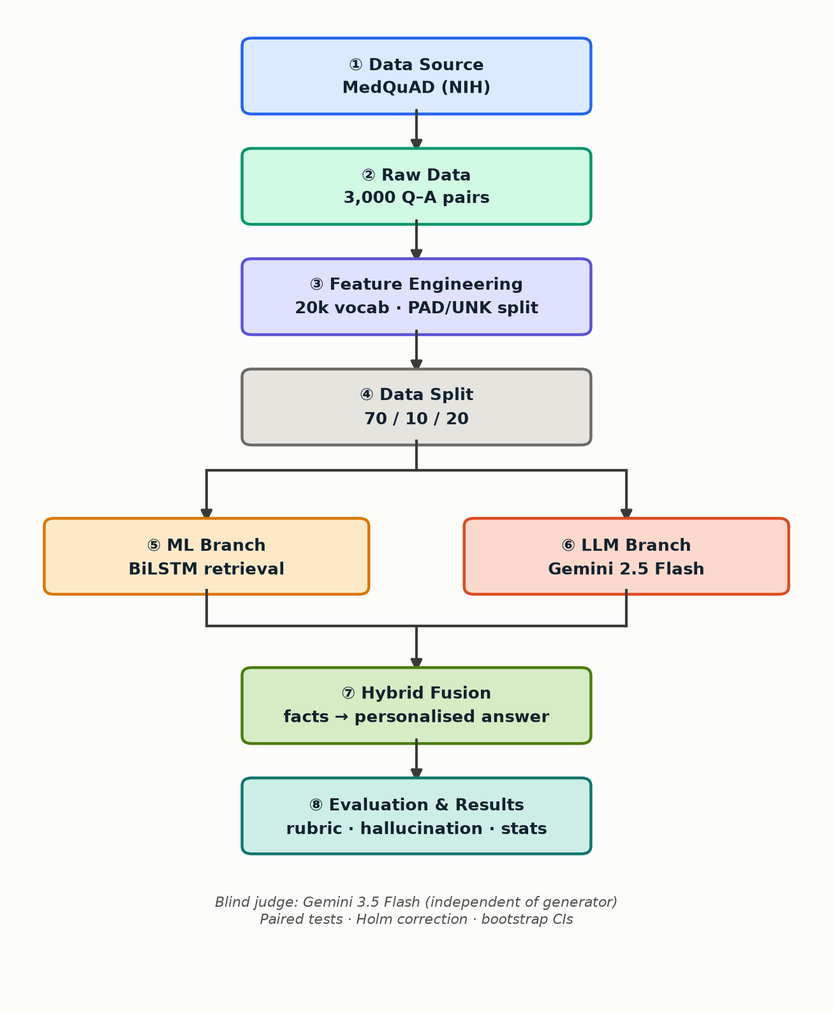
\includegraphics[width=0.40\textwidth]{fig-architecture.png}
\par\smallskip
\begingroup
\renewcommand{\thefigure}{4.1}
\refstepcounter{figure}
\label{fig:1}
\small\textbf{Figure \thefigure.} Eight-stage system architecture. Stages 5 and 6 process the same input independently, while Stage 7 combines their outputs.
\endgroup
\end{minipage}
\end{center}

\subsection{Retriever Specification}

Four retrieval methods were evaluated: TF-IDF with cosine similarity, Random Forest using TF-IDF features \citep{breiman2001}, TextCNN \citep{kim2014}, and a Siamese BiLSTM. The BiLSTM was selected because it achieved the best retrieval performance while remaining lightweight enough to train efficiently without GPU hardware. Although transformer-based retrievers such as Sentence-BERT \citep{reimers2019} may achieve higher accuracy, a smaller model was chosen because it is easier to analyse and debug.

The final retriever uses a single-layer bidirectional LSTM with 192 hidden units in each direction and 128-dimensional word embeddings. After masked mean pooling and L2 normalisation, each sentence is represented by a 384-dimensional embedding. A vocabulary of 20,000 words is used, with separate indices reserved for padding and unknown words. Questions are limited to 24 tokens and passages to 96 tokens. The model is trained using the InfoNCE objective with in-batch negatives, Adam optimisation, and eight training epochs.

During retrieval, the top 50 dense results are reranked using an equal combination of dense similarity and TF-IDF cosine similarity. A topic filter removes unrelated passages, while a facet bonus favours passages whose intent matches the user's question, improving retrieval precision.

\subsection{Prompt Design}

Both language-model systems use the same base prompt to ensure a fair comparison. The prompt instructs the assistant to generate patient-centred responses by referring to at least one existing medical condition or medication and organising the answer into three parts: a direct response, its relevance to the patient, and advice on when to seek medical attention.

Safety instructions prevent the model from suggesting medication dosages or making clinical diagnoses. The hybrid system includes one additional instruction requiring retrieved evidence to be used whenever available, while preventing unsupported numerical information from being generated. The retrieval process itself is never mentioned to the patient.

\subsection{Design Rationale}

The hybrid system was designed to combine the strengths of retrieval and language generation. Retrieval provides trustworthy supporting information but cannot personalise responses, while language models produce natural and personalised answers but may generate unsupported information. Combining both approaches aims to improve factual reliability without sacrificing readability.

The retriever first selects relevant medical evidence, which is summarised into key facts before being passed to the language model together with the patient profile. This two-stage process was adopted because early experiments showed that asking the model to process long retrieved passages and personalise responses simultaneously reduced personalisation quality.

Separating retrieval from generation also allows the knowledge base to be updated without retraining the language model. It additionally makes system errors easier to identify, as retrieval quality and response generation can be evaluated independently.

Finally, the design assumes that retrieval augmentation is beneficial only when relevant supporting information exists in the knowledge base. If retrieval returns unrelated documents, the language model cannot compensate for incorrect evidence. This assumption is evaluated experimentally in Section 7.4.

\section{Implementation}
\label{sec:Implementation}

This chapter describes the implementation of the proposed medical question answering system. The solution was developed in Python using PyTorch for the neural retriever, scikit-learn for retrieval and preprocessing, and Gemini for language generation. All experiments were performed on CPU, allowing the system to be trained and reproduced without specialised hardware.

\subsection{Retrieval Model}

The retrieval component is a Siamese BiLSTM encoder containing approximately 3.05 million trainable parameters. Unlike transformer-based retrievers, the model was trained from scratch, making its behaviour easier to analyse and reproduce.

During training, each question is paired with its correct answer while the remaining answers in the batch are treated as negative examples using the InfoNCE objective. This encourages the model to distinguish between semantically similar medical documents instead of relying on shared vocabulary alone. As a result, semantically related questions and answers are represented by nearby vector embeddings, allowing relevant passages to be retrieved even when different wording is used.

\subsection{Response Generation}

During inference, dense retrieval is combined with TF-IDF similarity to improve retrieval accuracy. The retrieved passages are filtered using the topic and intent constraints described in Chapter 4 before being passed to the language model.

Response generation is performed in two stages. The first stage extracts the medical facts relevant to the user's question, while the second generates a patient-focused response using these facts together with the patient profile. Restricting generated information to retrieved evidence improves factual reliability while allowing the language model to produce natural and personalised answers.

\subsection{Response Verification}

The generated responses are evaluated using two independent methods. First, Gemini 3.1 Flash Lite scores each response using the four-axis clinical rubric. To reduce evaluation bias, the judging model is different from the model used for generation, and responses are randomised before evaluation.

Second, every response is verified through claim-level analysis. Individual claims are compared with the supporting evidence, and numerical information such as medication doses and frequencies is checked for exact agreement. Using both methods provides an additional level of confidence in the reported results.

\section{Outputs Summary}
\label{sec:Outputs}

The outputs produced during this project are summarised in Table 3. Several of these outputs, particularly the evaluation framework and claim-level verification method, can be reused in future medical question answering research.

\refstepcounter{table}
\label{tab:3}
\begin{center}
\scriptsize
\setlength{\tabcolsep}{4pt}
\begin{tabular}{>{\raggedright\arraybackslash}p{0.177\textwidth}>{\raggedright\arraybackslash}p{0.127\textwidth}>{\raggedright\arraybackslash}p{0.400\textwidth}>{\raggedright\arraybackslash}p{0.189\textwidth}}
\toprule
\textbf{Output} & \textbf{Type} & \textbf{Description} & \textbf{Intended user} \\
\midrule
Trained retrieval model & Model & Siamese BiLSTM encoder reaching Recall@1 of 0.513 against 0.315 for the classical baseline, with the benchmark over 600 held-out questions. & Researchers reusing the encoder \\
Matched-prompt comparison protocol & Method & Design holding one base prompt constant across the augmented and unaugmented systems so retrieval is the only manipulated variable, run under two knowledge-base coverage conditions. & Researchers comparing RAG architectures \\
Scored response corpus & Annotated data & Answers from three systems to the same held-out questions, each scored on four axes and audited claim by claim. & Examiner, researchers \\
Evaluation instruments & Instruments & The four-axis clinical rubric, with the anchoring defect of Section 7.1 removed, and the non-LLM claim-level grounding audit. & Researchers evaluating clinical text \\
Working demonstrator & Artefact & Interactive prototype answering patient questions against a stored profile, used for the demonstration video. & Examiner, end users \\
Configuration manual & Document & Environment, data and execution details needed to reproduce every reported number; submitted separately from this report. & Examiner, researchers \\
\bottomrule
\end{tabular}
\end{center}

The project produced a trained BiLSTM retrieval model, a matched-prompt evaluation framework, a scored response dataset, reusable evaluation instruments, an interactive demonstration system, and a configuration manual containing the information required to reproduce the reported experiments.

\section{Evaluation and Critical Analysis}
\label{sec:Evaluation}

\subsection{Experiment 1: Evaluating the Assessment Method}

Before comparing the three systems, the evaluation method itself was examined because all subsequent results depend on it. The original evaluation rubric ended with a worked example containing the scores \textbf{24, 18, 20, and 16}, giving a total of \textbf{78}. During the initial evaluation, the Hybrid system received a score of 78 on 25 of the 30 questions, while the Gemini-only system received the same score on 15 questions.

To investigate whether the evaluation model was genuinely scoring responses or simply reproducing the example, three responses of different quality were evaluated five times at temperature zero using both the original rubric and a revised rubric containing placeholders and explicit scoring descriptors.

\par\medskip
\noindent\begin{minipage}{\textwidth}
\refstepcounter{table}
\label{tab:4}
\noindent\textbf{Table \thetable. Rubric anchoring ablation (five repeated evaluations at temperature 0)}\par
\medskip
\begin{center}
\small
\setlength{\tabcolsep}{5pt}
\begin{tabular}{>{\raggedright\arraybackslash}p{0.42\textwidth}>{\centering\arraybackslash}p{0.23\textwidth}>{\centering\arraybackslash}p{0.23\textwidth}}
\toprule
\textbf{Response quality} & \textbf{Old rubric (mean /100)} & \textbf{New rubric (mean /100)} \\
\midrule
Off-topic retrieved passage & \textbf{0.0} & \textbf{0.0} \\
Generic but clinically correct & \textbf{78.0} & \textbf{77.4} \\
Personalised, grounded and safe & \textbf{78.0} & \textbf{88.0} \\
\bottomrule
\end{tabular}
\end{center}
\end{minipage}
\par\medskip

The results show that the original rubric consistently limited high-quality responses to a maximum score of \textbf{78}, indicating that the evaluation model was influenced by the worked example instead of assessing response quality independently. Consequently, the previously reported difference between the Hybrid and Gemini-only systems (68.1 vs. 66.7) was not reliable. A paired statistical test produced \textbf{p = 0.766} with 13 exact ties, indicating no significant difference.

After replacing the worked example, the revised rubric produced a wider range of scores and removed the artificial ceiling. Because the evaluation was performed at temperature zero, all repeated runs produced identical results.

\subsection{Experiment 2: Retrieval Quality}

The second experiment evaluated the performance of the BiLSTM retriever. Five implementation issues were identified during development: pooling over padding tokens, mapping unknown words to the padding index, truncating passages to 50 tokens, training with a single random negative, and the absence of reranking. Together, these issues significantly reduced retrieval performance.

\par\medskip
\noindent\begin{minipage}{\textwidth}
\refstepcounter{table}
\label{tab:5}
\noindent\textbf{Table \thetable. Retrieval quality over the 3,000-document corpus (600 test questions)}\par
\medskip
\begin{center}
\small
\setlength{\tabcolsep}{5pt}
\begin{tabular}{>{\raggedright\arraybackslash}p{0.31\textwidth}>{\centering\arraybackslash}p{0.14\textwidth}>{\centering\arraybackslash}p{0.14\textwidth}>{\centering\arraybackslash}p{0.15\textwidth}>{\centering\arraybackslash}p{0.12\textwidth}}
\toprule
\textbf{Retriever} & \textbf{Recall@1} & \textbf{Recall@5} & \textbf{Recall@10} & \textbf{MRR} \\
\midrule
BiLSTM (original) & \textbf{0.010} & \textbf{0.035} & \textbf{0.073} & \textbf{0.034} \\
TF-IDF + cosine & \textbf{0.315} & \textbf{0.667} & \textbf{0.717} & \textbf{0.463} \\
BiLSTM (corrected) & \textbf{0.495} & \textbf{0.663} & \textbf{0.720} & \textbf{0.579} \\
BiLSTM + TF-IDF rerank & \textbf{0.513} & \textbf{0.743} & \textbf{0.788} & \textbf{0.620} \\
\bottomrule
\end{tabular}
\end{center}
\end{minipage}
\par\medskip

The original BiLSTM retriever achieved a \textbf{Recall@1 of 0.010}, compared with \textbf{0.315} for the TF-IDF baseline, indicating that the neural retriever performed substantially worse than the classical approach. After correcting the implementation issues, \textbf{Recall@1 increased to 0.495}, while TF-IDF reranking further improved it to \textbf{0.513} with an \textbf{MRR of 0.620}.

Overall, the corrected retriever outperformed the TF-IDF baseline by approximately \textbf{63\%} on Recall@1. These improvements also explain why the earlier Hybrid system generated more unsupported responses: the original retriever frequently returned irrelevant medical passages, which the language model then incorporated into its answers.

\subsection{Experiment 3: Three-System Comparison}

The primary experiment evaluated all three systems under \textbf{full knowledge-base coverage}. Table 6 summarises the results.

\par\medskip
\noindent\begin{minipage}{\textwidth}
\refstepcounter{table}
\label{tab:6}
\noindent\textbf{Table \thetable. Response quality under full knowledge-base coverage (n = 30)}\par
\medskip
\begin{center}
\footnotesize
\setlength{\tabcolsep}{3pt}
\begin{tabular}{>{\raggedright\arraybackslash}p{0.18\textwidth}>{\centering\arraybackslash}p{0.105\textwidth}>{\centering\arraybackslash}p{0.115\textwidth}>{\centering\arraybackslash}p{0.115\textwidth}>{\centering\arraybackslash}p{0.11\textwidth}>{\centering\arraybackslash}p{0.10\textwidth}>{\centering\arraybackslash}p{0.11\textwidth}}
\toprule
\textbf{System} & \textbf{Quality /100} & \textbf{Grounding /30} & \textbf{Personal. /25} & \textbf{Helpful. /25} & \textbf{Safety /20} & \textbf{Halluc. rate} \\
\midrule
Hybrid (BiLSTM + Gemini) & \textbf{79.27} & \textbf{24.47} & 15.87 & 20.07 & 18.87 & \textbf{0.767} \\
Gemini Only (LLM) & 78.23 & 20.87 & \textbf{18.20} & \textbf{20.37} & 18.80 & 0.913 \\
ML Only (BiLSTM + rules) & 48.97 & 20.60 & 2.77 & 10.57 & 15.03 & 0.133 \\
\bottomrule
\end{tabular}
\end{center}
\end{minipage}
\par\medskip

The Hybrid system achieved the highest overall quality score (\textbf{79.27}), followed closely by Gemini Only (\textbf{78.23}). Both language-model systems substantially outperformed the retrieval-only system (\textbf{48.97}), with the Hybrid exceeding ML Only by \textbf{30.3 points} (Cohen's $d$ = 1.15).

The comparison between the Hybrid and Gemini Only systems is more balanced. Although the Hybrid scored \textbf{1.03 points} higher overall, the difference was not statistically significant ($p$ = 0.55). The main advantage of the Hybrid lies in factual grounding, scoring \textbf{24.47} compared with \textbf{20.87}, while reducing the hallucination rate from \textbf{0.913} to \textbf{0.767}, a relative reduction of approximately \textbf{16\%}. In contrast, Gemini Only achieved a higher personalisation score (\textbf{18.20} vs. \textbf{15.87}).

These results suggest that retrieval mainly improves factual grounding, whereas the standalone language model produces more personalised responses. As a result, overall quality alone does not fully reflect the strengths of each system.

\begin{center}
\begin{minipage}{\textwidth}
\centering
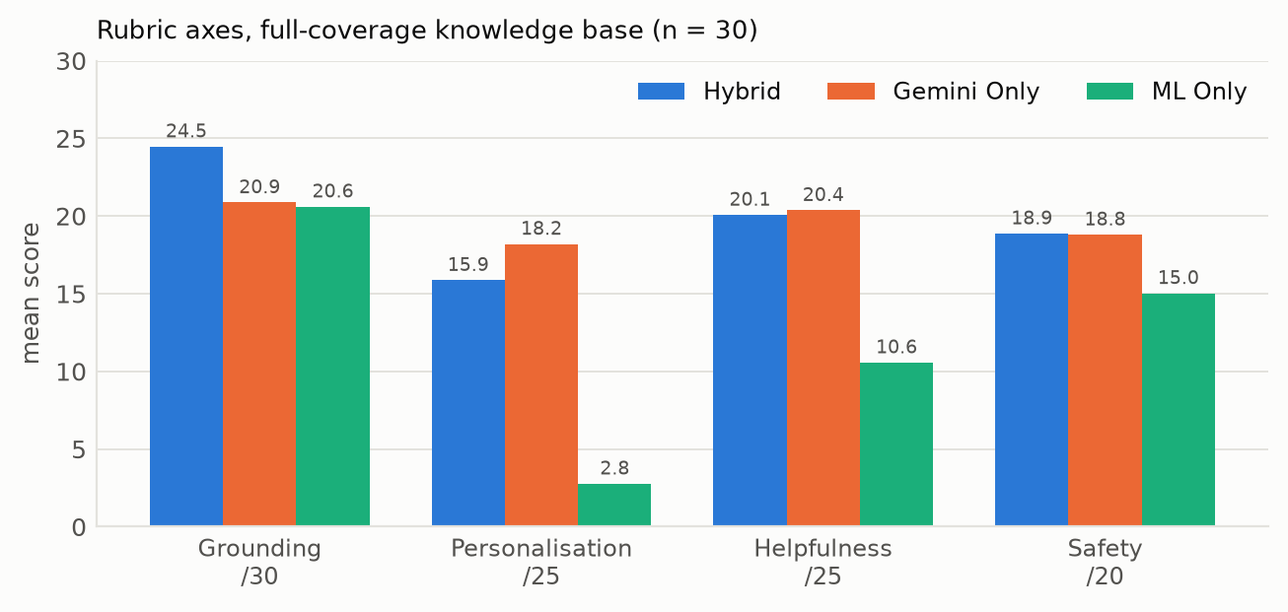
\includegraphics[width=0.88\textwidth]{fig-quality-axes.png}
\par\smallskip
\begingroup
\renewcommand{\thefigure}{7.1}
\refstepcounter{figure}
\label{fig:2}
\small\textbf{Figure \thefigure.} Per-axis rubric scores for the three systems under full knowledge-base coverage.
\endgroup
\end{minipage}
\end{center}

The retrieval-only system achieved the lowest overall score but recorded the smallest hallucination rate (\textbf{0.133}) because it only returns retrieved information. However, its very low personalisation score (\textbf{2.77}) shows that it cannot adapt responses to individual patients.

\subsection{Experiment 4: Knowledge-Base Coverage Ablation}

The second experiment evaluated system performance after removing the correct source document from the knowledge base. The results are presented in Table 7.

\par\medskip
\noindent\begin{minipage}{\textwidth}
\refstepcounter{table}
\label{tab:7}
\noindent\textbf{Table \thetable. Response quality under leave-one-out knowledge-base coverage (n = 30)}\par
\medskip
\begin{center}
\footnotesize
\setlength{\tabcolsep}{3pt}
\begin{tabular}{>{\raggedright\arraybackslash}p{0.18\textwidth}>{\centering\arraybackslash}p{0.105\textwidth}>{\centering\arraybackslash}p{0.115\textwidth}>{\centering\arraybackslash}p{0.115\textwidth}>{\centering\arraybackslash}p{0.11\textwidth}>{\centering\arraybackslash}p{0.10\textwidth}>{\centering\arraybackslash}p{0.11\textwidth}}
\toprule
\textbf{System} & \textbf{Quality /100} & \textbf{Grounding /30} & \textbf{Personal. /25} & \textbf{Helpful. /25} & \textbf{Safety /20} & \textbf{Halluc. rate} \\
\midrule
Gemini Only (LLM) & \textbf{78.70} & 22.47 & \textbf{17.40} & 20.37 & 18.47 & 0.891 \\
Hybrid (BiLSTM + Gemini) & 78.10 & \textbf{22.67} & 16.63 & 20.10 & 18.70 & \textbf{0.889} \\
ML Only (BiLSTM + rules) & 29.53 & 12.27 & 1.37 & 3.63 & 12.27 & 0.200 \\
\bottomrule
\end{tabular}
\end{center}
\end{minipage}
\par\medskip

Removing the correct document had little effect on the two language-model systems. Gemini Only scored \textbf{78.70}, while the Hybrid achieved \textbf{78.10}, meaning the small advantage observed under full coverage disappeared. In contrast, the retrieval-only system dropped from \textbf{48.97} to \textbf{29.53}, showing that it depends heavily on the availability of relevant documents.

The main effect is seen in grounding and hallucination. Under full coverage, the Hybrid achieved a \textbf{3.60-point} improvement in grounding and reduced hallucinations by \textbf{16\%}. When the correct document was removed, grounding scores became almost identical (\textbf{22.67} vs. \textbf{22.47}) and hallucination rates were also nearly the same (\textbf{0.889} vs. \textbf{0.891}). This indicates that retrieval augmentation is beneficial only when the knowledge base contains relevant evidence.

\begin{center}
\begingroup
\renewcommand{\thefigure}{7.2}
\refstepcounter{figure}
\label{fig:3}
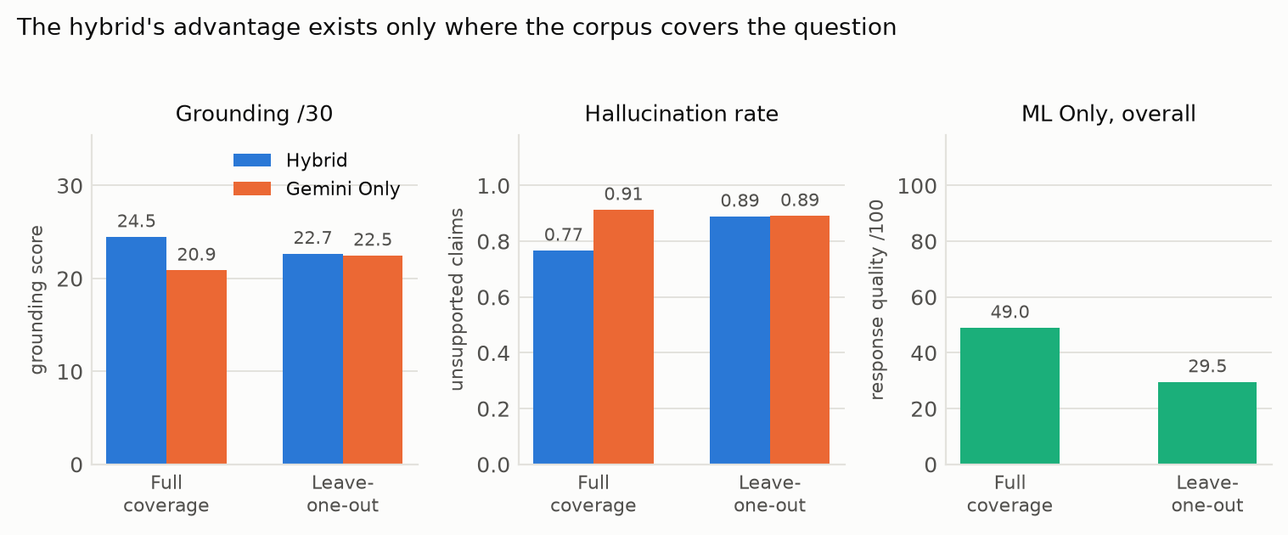
\includegraphics[width=0.94\textwidth]{fig-coverage.png}
\endgroup
\end{center}

Overall, the coverage experiment confirms that retrieval augmentation improves factual reliability only when relevant documents are available. When the required evidence is missing, the Hybrid behaves similarly to the standalone language model, while the retrieval-only system performs considerably worse.

\subsection{Experiment 5: Efficiency and Computational Cost}

System quality alone does not determine whether it is suitable for practical use. This experiment evaluates the computational cost of each architecture, including retrieval time, total response time, answer length, and response quality.

\par\medskip
\noindent\begin{minipage}{\textwidth}
\refstepcounter{table}
\label{tab:8}
\noindent\textbf{Table \thetable. Cost profile of the three architectures}\par
\medskip
\begin{center}
\footnotesize
\setlength{\tabcolsep}{3pt}
\begin{tabular}{>{\raggedright\arraybackslash}p{0.16\textwidth}>{\centering\arraybackslash}p{0.085\textwidth}>{\centering\arraybackslash}p{0.13\textwidth}>{\centering\arraybackslash}p{0.13\textwidth}>{\centering\arraybackslash}p{0.125\textwidth}>{\centering\arraybackslash}p{0.095\textwidth}>{\centering\arraybackslash}p{0.14\textwidth}}
\toprule
\textbf{System} & \textbf{Model Calls} & \textbf{Local Retrieval (ms)} & \textbf{End-to-End (ms)} & \textbf{Answer Length (words)} & \textbf{Quality /100} & \textbf{\shortstack{Hallucination\\Rate}} \\
\midrule
ML Only (BiLSTM + rules) & 0 & 11 & 11 & 81 & 49.0 & 0.133 \\
Gemini Only (LLM) & 1 & 0 & 1497 & 160 & 78.2 & 0.913 \\
Hybrid (BiLSTM + Gemini) & 2 & 11 & 1926 & 148 & 79.3 & 0.767 \\
\bottomrule
\end{tabular}
\end{center}
\end{minipage}
\par\medskip

The BiLSTM retriever completed retrieval in a median of \textbf{11 ms}, representing only \textbf{0.6\%} of the Hybrid system's total response time. This indicates that retrieval itself adds very little computational cost, with most of the latency coming from the language model.

The Hybrid system required \textbf{1926 ms}, compared with \textbf{1497 ms} for Gemini Only, making it approximately \textbf{29\%} slower because of the additional generation stage. In return, the Hybrid reduced unsupported clinical statements from \textbf{3.43} to \textbf{2.73} per response, improving factual reliability.

The ML Only system was the fastest, generating responses in \textbf{11 ms} without external API calls. It also achieved the lowest hallucination rate (\textbf{0.133}). However, this came at the cost of very limited personalisation, demonstrating that computational efficiency alone is insufficient for high-quality patient-centred responses.

\subsection{Statistical Significance and Effect Sizes}

Table 9 presents the statistical comparison between the three systems under full knowledge-base coverage.

\par\medskip
\noindent\begin{minipage}{\textwidth}
\refstepcounter{table}
\label{tab:9}
\noindent\textbf{Table \thetable. Pairwise statistical comparisons (n = 30)}\par
\medskip
\begin{center}
\scriptsize
\setlength{\tabcolsep}{3pt}
\begin{tabular}{>{\raggedright\arraybackslash}p{0.16\textwidth}>{\centering\arraybackslash}p{0.11\textwidth}>{\centering\arraybackslash}p{0.12\textwidth}>{\centering\arraybackslash}p{0.14\textwidth}>{\centering\arraybackslash}p{0.12\textwidth}>{\centering\arraybackslash}p{0.09\textwidth}>{\raggedright\arraybackslash}p{0.12\textwidth}}
\toprule
\textbf{Comparison} & \textbf{Mean Difference} & \textbf{Paired $t$ ($p$)} & \textbf{Holm-adjusted $p$} & \textbf{Wilcoxon ($p$)} & \textbf{Cohen's $d$} & \textbf{Verdict} \\
\midrule
Hybrid vs Gemini Only & +1.03 & 0.5471 & 0.5471 & 0.7843 & 0.11 & Not significant \\
Hybrid vs ML Only & +30.30 & $7.3 \times 10^{-7}$ & $2.2 \times 10^{-6}$ & $5.7 \times 10^{-6}$ & 1.15 & Significant \\
Gemini Only vs ML Only & +29.27 & $1.3 \times 10^{-6}$ & $2.6 \times 10^{-6}$ & $5.2 \times 10^{-6}$ & 1.11 & Significant \\
\bottomrule
\end{tabular}
\end{center}
\end{minipage}
\par\medskip

The results show that both language-model systems significantly outperform the retrieval-only system. However, the 1.03-point difference between the Hybrid and Gemini Only systems is not statistically significant. Although the Hybrid achieved the highest overall score, the available sample size was insufficient to demonstrate a reliable difference.

The results therefore support one clear conclusion: retrieval augmentation improves factual reliability, while the overall quality difference between the Hybrid and standalone language model cannot be confirmed statistically.

\subsection{Qualitative Analysis: One Question, Three Systems}

Overall evaluation scores do not fully explain how the systems behave. Table 10 presents one representative example in which all three systems answered the same question, \textbf{``What is Nephrocalcinosis?}

\par\medskip
\noindent\begin{minipage}{\textwidth}
\refstepcounter{table}
\label{tab:10}
\noindent\textbf{Table \thetable. Example responses from the three systems}\par
\medskip
\begin{center}
\scriptsize
\setlength{\tabcolsep}{3pt}
\begin{tabular}{>{\raggedright\arraybackslash}p{0.09\textwidth}>{\raggedright\arraybackslash}p{0.36\textwidth}>{\centering\arraybackslash}p{0.10\textwidth}>{\centering\arraybackslash}p{0.135\textwidth}>{\centering\arraybackslash}p{0.115\textwidth}>{\centering\arraybackslash}p{0.07\textwidth}}
\toprule
\textbf{System} & \textbf{Opening of Response (Excerpt)} & \textbf{Grounding} & \textbf{Personal\-isation} & \textbf{Hallucina\-tion} & \textbf{Total} \\
\midrule
ML Only & ``Nephrocalcinosis is a disorder in which there is excess calcium deposited in the kidneys... This is general information, not advice.'' & 30 / 30 & 5 / 25 & 0.00 & 68 \\
Gemini Only & ``Calcium deposits build up within the tiny structures of your kidneys... For a 45-year-old like you managing diabetes and hypertension with metformin and lisinopril, protecting kidney function is especially critical.'' & 26 / 30 & 20 / 25 & 0.75 & 88 \\
Hybrid & ``Excess deposition of calcium within the substance of the kidneys. People who have this condition may not experience any symptoms initially... For a 45-year-old living with diabetes and hypertension, your kidneys are already working hard.'' & 30 / 30 & 18 / 25 & 0.40 & 90 \\
\bottomrule
\end{tabular}
\end{center}
\end{minipage}
\par\medskip

The example illustrates the strengths and weaknesses of each approach. The retrieval-only system provides accurate information but offers little personalisation. Gemini Only generates a personalised response but includes claims that are not fully supported by the available evidence. The Hybrid combines both approaches by grounding the response in retrieved medical information while still relating the explanation to the patient's condition.

Although this example alone does not prove the overall findings, it clearly demonstrates the behavioural differences identified throughout the quantitative evaluation.

\subsection{Answering the Research Question}

The results show that the Hybrid system achieves the highest overall quality only when the knowledge base contains relevant information, and even then the improvement over the standalone language model is not statistically significant. However, the Hybrid consistently produces more faithful responses by improving grounding and reducing unsupported claims.

When the relevant document is removed from the knowledge base, the Hybrid no longer outperforms the standalone language model. This indicates that the benefits of retrieval augmentation depend on knowledge-base coverage. Therefore, the main contribution of retrieval is improved factual reliability rather than higher overall response quality.

\subsection{Limitations}

Several limitations should be considered when interpreting these findings.

First, the evaluation uses only \textbf{30} test questions. With an observed standard deviation of approximately \textbf{25} points, the Hybrid's \textbf{1.03-point} advantage over the language model is too small to detect reliably. In contrast, the differences between both language-model systems and the retrieval-only system are much larger and statistically detectable.

Second, prompt wording and retrieval parameters were refined using an initial subset of the test data before evaluation on a separate held-out subset. Although this reduces bias in the reported results, future work should validate the approach using additional medical datasets.

Finally, the experiments use a single simulated patient profile. This isolates the effect of personalisation but limits the generalisability of the findings to patients with different medical histories or conditions.

\section{Discussion}
\label{sec:Discussion}

\subsection{Answering the Research Question}

This study investigated whether combining a BiLSTM retriever with a large language model improves personalised medical question answering. The results show that the Hybrid system achieved the highest overall quality only when the knowledge base contained relevant information. Although the improvement over the standalone language model was not statistically significant, the Hybrid consistently produced more faithful responses by improving grounding and reducing unsupported claims.

When the relevant document was removed from the knowledge base, the Hybrid no longer outperformed the language model. This confirms that retrieval augmentation is effective only when suitable supporting evidence is available. Overall, retrieval improves factual reliability rather than overall response quality.

\subsection{Discussion of Findings}

The findings are generally consistent with previous studies. \citet{shuster2021} reported that retrieval augmentation reduces hallucinations, and this study observed a similar \textbf{16\% reduction} in unsupported medical claims. Likewise, \citet{xiong2024} found that the effectiveness of medical RAG depends on knowledge-base coverage, which was confirmed through the leave-one-out experiment.

One important observation differs from earlier work. Although retrieval improved grounding, it slightly reduced personalisation because the language model devoted more attention to retrieved evidence than to the patient profile. This trade-off suggests that retrieval augmentation improves factual reliability but does not automatically improve every aspect of response quality.

The study also highlights the importance of reliable evaluation methods. The initial evaluation rubric introduced an anchoring effect that influenced the scoring process, demonstrating that LLM-based evaluation should be carefully designed and supported by independent verification methods.

\subsection{Limitations}

Several limitations should be considered when interpreting the findings.

First, the evaluation included only \textbf{30} test questions, limiting the statistical power of the comparison between the Hybrid and standalone language model. Second, prompt design and retrieval parameters were refined before the final evaluation, although testing was performed on a separate held-out subset. Finally, the study used a single simulated patient profile, which limits the generalisability of the personalisation results. Future studies should evaluate a wider range of patient profiles and medical datasets.

\section{Conclusion and Future Work}
\label{sec:Conclusion}

\subsection{Conclusion}

This study compared three approaches for personalised medical question answering: a retrieval-only system, a standalone large language model, and a Retrieval-Augmented Generation (RAG) hybrid. The results showed that the Hybrid system produced the most faithful responses when the knowledge base contained relevant information, while the retrieval-only system remained the fastest and most factually constrained. However, the overall quality difference between the Hybrid and standalone language model was not statistically significant.

The study also demonstrated that correcting the neural retriever substantially improved retrieval performance and highlighted the importance of carefully designing LLM-based evaluation methods. Overall, the findings suggest that retrieval augmentation is most valuable for improving factual reliability rather than overall response quality.

\subsection{Future Work}

Future work should evaluate the system using larger medical datasets and a broader range of patient profiles. Replacing the BiLSTM retriever with biomedical embedding models such as BioBERT or Sentence-BERT may further improve retrieval quality. Another promising direction is to introduce retrieval-confidence estimation so that the system can automatically determine when retrieval should be used and when a standalone language model is more appropriate. Finally, evaluation by healthcare professionals would provide additional evidence of the clinical usefulness of the proposed system.

\nocite{asai2024}



%% --------------------
%% |   Bibliography   |
%% --------------------

% Use dcu for Harvard references --> Make sure to use correctly the citep and citet commands
\bibliographystyle{dcu}

% Use IEEEtran for numeric references (but you will need to comment natbib package, change citep/citet commands to cite, and manually type the first author last name where needed.
%\bibliographystyle{IEEEtran}

\bibliography{refs}

\end{document}
